%%%%%%%%%%%%%%%%%%%%%%%%%%%%%%%%%%%%%%%%%%%%%%%%%%%%%%%%%%%%%%%%%%%%%%%%%%%%%%%%
% File coling2014.tex
%
% Contact: jwagner@computing.dcu.ie
%
% Based on the style files for ACL-2014, which were, in turn,
% Based on the style files for ACL-2013, which were, in turn,
% Based on the style files for ACL-2012, which were, in turn,
% based on the style files for ACL-2011, which were, in turn, 
% based on the style files for ACL-2010, which were, in turn, 
% based on the style files for ACL-IJCNLP-2009, which were, in turn,
% based on the style files for EACL-2009 and IJCNLP-2008...
%
% Based on the style files for EACL 2006 by  e.agirre@ehu.es or
% Sergi.Balari@uab.es and that of ACL 08 by Joakim Nivre and Noah Smith

\documentclass[11pt]{article}
\usepackage{coling2014}
\usepackage{times}
\usepackage{url}
\usepackage{latexsym}

%\setlength\titlebox{5cm}

\usepackage[utf8]{inputenc}
\usepackage{amsmath}
\usepackage{relsize}
\usepackage{xfrac}
\usepackage{booktabs}
\usepackage{multirow}
\usepackage{rotating}
\usepackage{lipsum}
\usepackage{color}
\usepackage{subfigure}
\usepackage{overpic}

\newtheorem{property}{Property}
\newcommand\TODO[1]{\textcolor{red}{[TODO #1]}}

\title{Candidate Extraction Impact on Automatic Keyphrase Extraction}

\author{
  Adrien Bougouin \and Florian Boudin \and Béatrice Daille\\
  Université de Nantes, LINA, France\\
  {\tt \{adrien.bougouin,florian.boudin,beatrice.daille\}@univ-nantes.fr}
}

\date{}

\begin{document}
  \maketitle
  \begin{abstract}
    Keyphrase extraction is the task of identifying single or multi-word
    expressions that best represent the content of a document. A wide range of
    methods are proposed to automatically extract keyphrases. Regardless the
    differences between them, we observe common steps. Among these steps, the
    most important ones are the extraction of keyphrase candidates and the
    classification, or ranking of them. Many methods about the core problem of
    classifying, or ranking, the keyphrase candidates are proposed, but no work
    dedicated to the analysis of the impact of the various candidate extraction
    methods has been done and researchers have to make (again) observations that
    should be stated once and for all. In this paper, we present the common
    candidate extraction methods and show their impact on different keyphrase
    extraction methods.%, which belong to different categories.
  \end{abstract}

  \section{Introduction}
\label{sec:section}
  Keyphrases are single or multi-word expressions that represent the main topics
  of a document. Keyphrases are useful in many tasks such as information
  retrieval~\cite{medelyan2008smalltrainingset}, document
  summarization~\cite{litvak2008graphbased} or document
  clustering~\cite{han2007webdocumentclustering}. Although scientific articles
  usually provide them, most of the documents have no associated keyphrases.
  Therefore, the problem of automatically assigning keyphrases to documents is
  an active field of research.

  \todo[inline]{Introduire free indexing et controlled indexing}
  Automatic keyphrase extraction methods are divided into two categories:
  supervised and unsupervised methods. Supervised methods typically recast
  keyphrase extraction as a binary classification
  task~\cite{witten1999kea,sujian2003maximumentropy,eichler2010keywe}. For
  unsupervised methods, keyphrase extraction is often considered as a ranking
  task and many approaches are
  used~\cite{barker2000nounphrasehead,tomokiyo2003languagemodel,mihalcea2004textrank}.
  As distinct as they are, both supervised and unsupervised methods rely on a
  preliminary candidate extraction step which identifies single and multi-word
  expressions that have the same syntactic properties than a keyphrase. These
  expressions are the only textual units that can be extracted as keyphrases.
  
  In this paper, we focus on the candidate extraction step and show its impact
  on the performance of automatic keyphrase extraction. Various methods
  are commonly employed to extract keyphrase candidates. Usually, a set of
  either single words, n-grams filtered by stop words, NP-chunks or sequences of
  words matching given patterns is extracted~\cite{hulth2003keywordextraction}.
  According to the chosen method, the extracted set contains more or less
  candidates, and the amount of these that match with the ground truth
  keyphrases may vary. Hence, a few questions arise. How the different sets
  influence the keyphrase extraction? Do large candidate sets introduce noise
  that affects the performance of some keyphrase extraction methods?

  We seek to better understand the impact of candidate extraction methods on
  keyphrase extraction by studying the aforementioned questions. We first
  quantify the differences between the candidate sets obtained by the commonly
  used methods. Also, we propose to use another method developed to extract
  noun-phrases for document indexing~\cite{evans1996nounphraseanalysis} and we
  argue that such term detection
  method~\cite{castellvi2001automatictermdetection} provides solid keyphrase
  candidates. Then, we evaluate the impact of the candidate extraction methods
  on three dissimilar keyphrase extraction methods. We select
  KEA~\cite{witten1999kea} to represent supervised methods,
  TF-IDF~\cite{jones1972tfidf} to represent unsupervised methods that require a
  collection of documents and TopicRank~\cite{bougouin2013topicrank} to
  represent unsupervised methods that only make use of the document to analyse.

  \todo[inline]{Results show that...}

\section{Definition of candidate Keyphrases}
\label{sec:study_of_ground_truth_keyphrases}
  Candidate keyphrases are textual units which can be selected as keyphrases
  for a document they are extracted from. Hence, they must have the same
  syntactic and linguistic properties than ground truth keyphrases. This section
  aims to determine those properties by analysing three standard evaluation
  datasets, for keyphrase extraction, and by providing statistics about
  reference keyphrases (ground truth keyphrases).

  \subsection{Keyphrase extraction datasets}
  \label{subsec:keyphrase_extraction_datasets}
    Keyphrase extraction datasets are used to evaluate or train keyphrase
    extraction methods. Hence, the datasets are collections of documents paired
    with reference keyphrases, given by authors, readers or both.
    % TODO unrestricted to the content of the document.
    \todo[inline]{Présentation générale des corpus pour l'extraction de
                  termes-clés.}
    \todo[inline]{Présentation des corpus qui seront utilisés}

  \subsection{Keyphrase analysis}
  \label{subsec:keyphrase_analysis}
    \begin{table*}[h]
      \centering
      \begin{tabular}{@{~}r@{~~}r@{~~}c@{~~}c@{~~}c@{~}}
        \toprule
        & \multirow{2}{*}[-2pt]{\textbf{Statistics}} & \multicolumn{3}{c}{\textbf{Corpora}}\\
        \cmidrule{3-5}
        & & DUC & SemEval & DEFT\\
        \midrule
        \multirow{6}{*}[-2pt]{\begin{sideways}\textbf{Documents}\end{sideways}} & Language & English & English & French\\
        & Type & News & Papers & Papers\\
        & Documents & 208 & 144 & 141\\
        & Tokens/document & & 5134.6 & 7276.7\\
        & Keyphrases/document & 8.1 & 15.4 & 5.4\\
        & Missings keyphrases & & 13.5\% & 18.2\%\\
        \addlinespace[\defaultaddspace]
        \multirow{10}{*}[-2pt]{\begin{sideways}\textbf{Keyphrases}\end{sideways}} & Unigrams & 26.2\% & 20.2\% & 66.4\%\\
        & Bigrams & 54.1\% & 53.4\% & 20.7\%\\
        & Trigrams and more & 19.7\% & 26.4\% & 12.9\%\\
        & Containing nouns & 99.5\% & 98.8\% & 95.5\%\\
        & Containing adjectives & 41.6\% & 40.5\% & 28.8\%\\
        & Containing verbs & $~~$0.9\% & $~~$3.4\% & $~~$0.5\%\\
        & Containing adverbs & $~~$1.3\% & $~~$0.6\% & $~~$0.5\%\\
        & Containing prepositions & $~~$0.2\% & $~~$1.2\% & 12.7\%\\
        & Containing determiners & $~~$0.0\% & $~~$0.0\% & $~~$8.1\%\\
        & Containing others & $~~$1.3\% & $~~$2.1\% & $~~$5.8\%\\
        \bottomrule
      \end{tabular}
      \caption{Dataset statistics. The missing keyphrase percentage is
               determined based on the stemmed form of the gold standard
               keyphrases. \label{tab:dataset_statistics}}
    \end{table*}

    \todo[inline]{Donner les séquences de POS les plus fréquentes dans le gold
                  standard.}

\section{Candidate Extraction}
\label{sec:candidate_extraction}
  \todo[inline]{Objectif + pré-requis.}

  \subsection{N-Gram Extraction}
  \label{subsec:n_gram_extraction}
  \subsection{NP-Chunk Extraction}
  \label{subsec:np_chunk_extraction}
  \subsection{Pattern Matching}
  \label{subsec:pattern_matching}
  \subsection{Term Extraction}
  \label{subsec:term_extraction}

\section{Keyphrase Extraction}
\label{sec:keyphrase_extraction}
  \todo[inline]{Fonctionnement général.}
  \begin{figure}
    \centering
    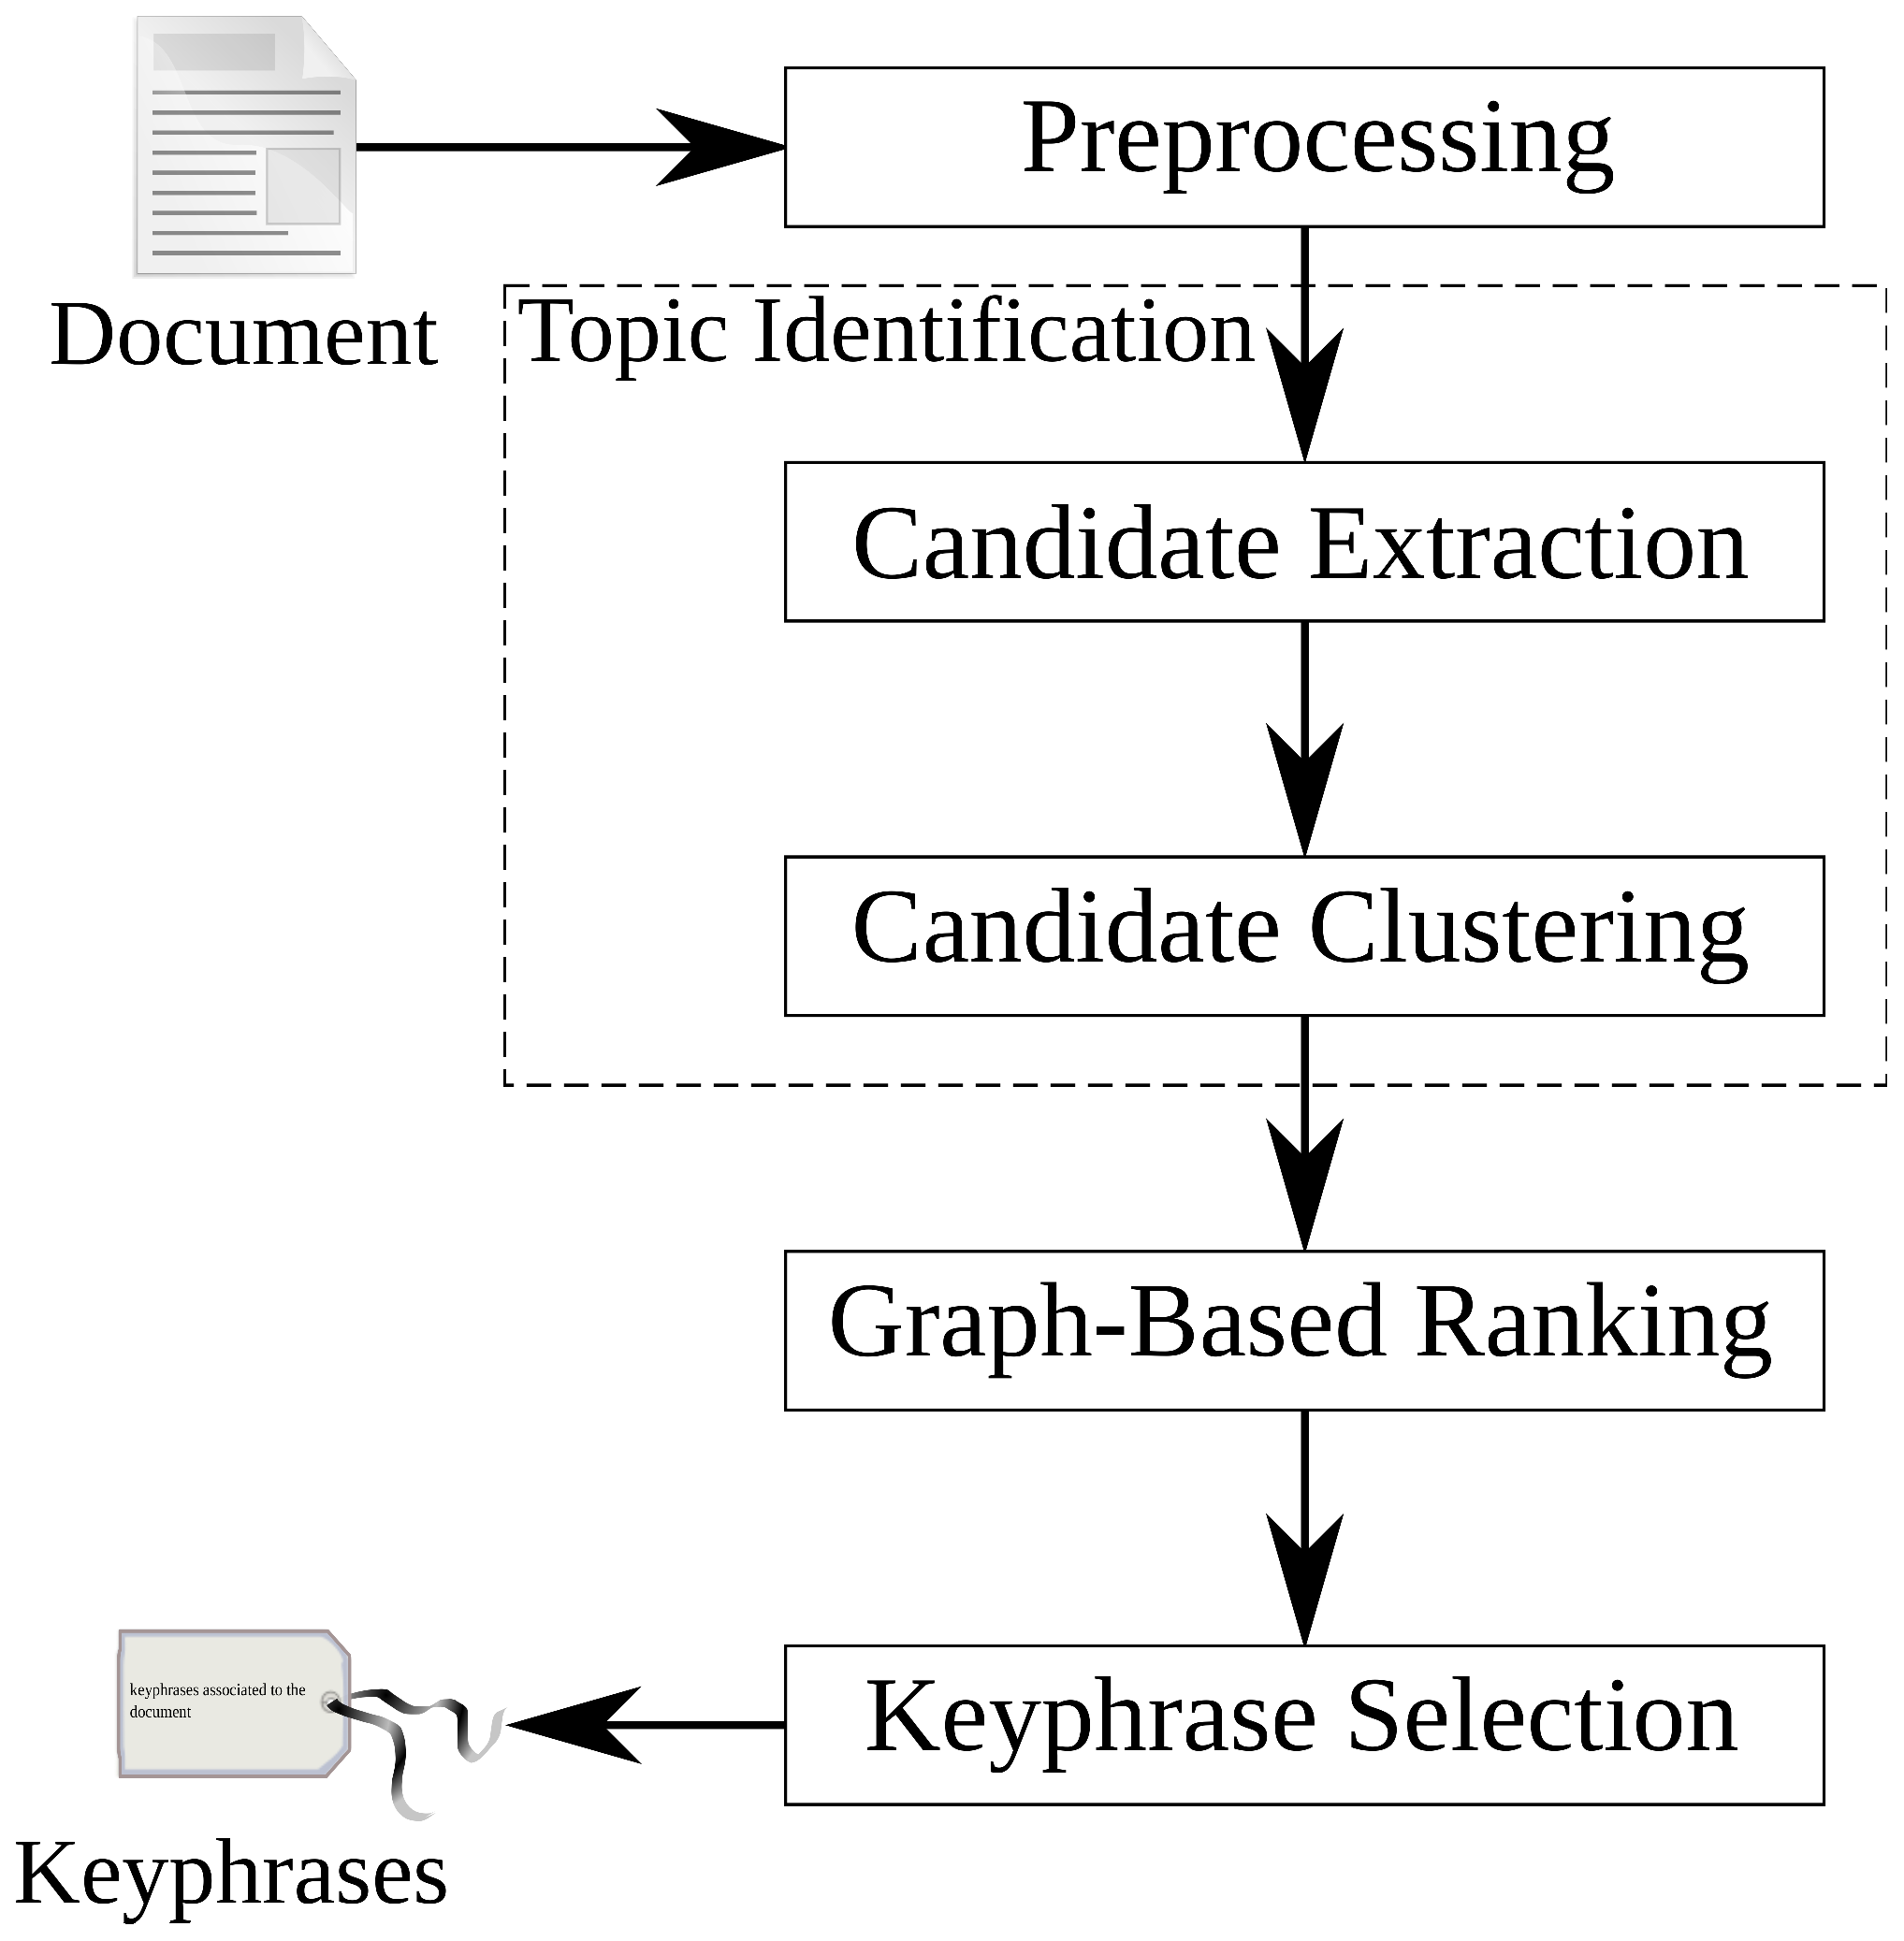
\includegraphics[width=0.3\textwidth]{include/processing_steps.eps}
    \caption{Processing steps of automatic keyphrase extraction methods.
             \label{fig:processing_steps}}
  \end{figure}

  \subsection{TF-IDF}
  \label{subsec:tfidf}
  \subsection{TopicRank}
  \label{subsec:topicrank}
  \subsection{KEA}
  \label{subsec:kea}

\section{Evaluation}
\label{sec:evaluation}
  \todo[inline]{Expliquer les deux évaluations: intrinsèque et extrinsèque.}

  \subsection{Experimental Setting}
  \label{subsec:experimental_setting}

  \subsection{Candidate Extraction}
  \label{subsec:candidate_extraction}
    \todo[inline]{Donner le rappel max et comparer avec la taille des différents
                  ensemble.}

    \begin{table}[h]
      \centering
      \begin{tabular}{@{~}r@{~~}c@{~~}c@{~~}c@{~~}c@{~}}
        \toprule
        \multirow{2}{*}[-2pt]{\textbf{Methods}} & \multicolumn{2}{c}{\textbf{DUC}} & \multicolumn{2}{c}{\textbf{SemEval}}\\
        \cmidrule(r){2-3}\cmidrule{4-5}
        & Candidates & Rmax & Candidates & Rmax\\
        \midrule
        1-grams\\
        2-grams\\
        3-grams\\
        4-grams\\
        5-grams\\
        Chunks\\
        Patterns1\\
        Patterns2\\
        Terms\\
        \bottomrule
      \end{tabular}
      \caption{Candidate extraction statistics.
               \label{tab:candidate_extraction_statistics}}
    \end{table}

    \todo[inline]{Quels sont les termes candidats communs aux ensembles, les
                  propriétés ?}

  \subsection{Keyphrase Extraction}
  \label{subsec:keyphrase_extraction}
    \todo[inline]{Quelles sont les performances de chaque méthode avec chaque
                  ensemble de termes candidats ?}

    \begin{table}[h]
      \centering
      \begin{tabular}{@{~}r@{~~}c@{~~}c@{~~}c@{~~}c@{~~}c@{~~}c@{~}}
        \toprule
        \multirow{2}{*}[-2pt]{\textbf{Methods}} & \multicolumn{3}{c}{\textbf{DUC}} & \multicolumn{3}{c}{\textbf{SemEval}}\\
        \cmidrule(r){2-4}\cmidrule{5-7}
        & P & R & F & P & R & F\\
        \midrule
        \multicolumn{1}{l}{\textbf{TF-IDF}}\\
        1-grams & ${~~}$00.0 & ${~~}$00.0 & ${~~}$00.0 & ${~~}$00.0 & ${~~}$00.0 & ${~~}$00.0\\
        2-grams & ${~~}$00.0 & ${~~}$00.0 & ${~~}$00.0 & ${~~}$00.0 & ${~~}$00.0 & ${~~}$00.0\\
        3-grams & ${~~}$00.0 & ${~~}$00.0 & ${~~}$00.0 & ${~~}$00.0 & ${~~}$00.0 & ${~~}$00.0\\
        4-grams & ${~~}$00.0 & ${~~}$00.0 & ${~~}$00.0 & ${~~}$00.0 & ${~~}$00.0 & ${~~}$00.0\\
        5-grams & ${~~}$00.0 & ${~~}$00.0 & ${~~}$00.0 & ${~~}$00.0 & ${~~}$00.0 & ${~~}$00.0\\
        Chunks & ${~~}$00.0 & ${~~}$00.0 & ${~~}$00.0 & ${~~}$00.0 & ${~~}$00.0 & ${~~}$00.0\\
        Patterns1 & ${~~}$00.0 & ${~~}$00.0 & ${~~}$00.0 & ${~~}$00.0 & ${~~}$00.0 & ${~~}$00.0\\
        Patterns2 & ${~~}$00.0 & ${~~}$00.0 & ${~~}$00.0 & ${~~}$00.0 & ${~~}$00.0 & ${~~}$00.0\\
        Terms & ${~~}$00.0 & ${~~}$00.0 & ${~~}$00.0 & ${~~}$00.0 & ${~~}$00.0 & ${~~}$00.0\\
        \multicolumn{1}{l}{\textbf{TopicRank}}\\
        1-grams & ${~~}$00.0 & ${~~}$00.0 & ${~~}$00.0 & ${~~}$00.0 & ${~~}$00.0 & ${~~}$00.0\\
        2-grams & ${~~}$00.0 & ${~~}$00.0 & ${~~}$00.0 & ${~~}$00.0 & ${~~}$00.0 & ${~~}$00.0\\
        3-grams & ${~~}$00.0 & ${~~}$00.0 & ${~~}$00.0 & ${~~}$00.0 & ${~~}$00.0 & ${~~}$00.0\\
        4-grams & ${~~}$00.0 & ${~~}$00.0 & ${~~}$00.0 & ${~~}$00.0 & ${~~}$00.0 & ${~~}$00.0\\
        5-grams & ${~~}$00.0 & ${~~}$00.0 & ${~~}$00.0 & ${~~}$00.0 & ${~~}$00.0 & ${~~}$00.0\\
        Chunks & ${~~}$00.0 & ${~~}$00.0 & ${~~}$00.0 & ${~~}$00.0 & ${~~}$00.0 & ${~~}$00.0\\
        Patterns1 & ${~~}$00.0 & ${~~}$00.0 & ${~~}$00.0 & ${~~}$00.0 & ${~~}$00.0 & ${~~}$00.0\\
        Patterns2 & ${~~}$00.0 & ${~~}$00.0 & ${~~}$00.0 & ${~~}$00.0 & ${~~}$00.0 & ${~~}$00.0\\
        Terms & ${~~}$00.0 & ${~~}$00.0 & ${~~}$00.0 & ${~~}$00.0 & ${~~}$00.0 & ${~~}$00.0\\
        \multicolumn{1}{l}{\textbf{KEA}}\\
        1-grams & ${~~}$00.0 & ${~~}$00.0 & ${~~}$00.0 & ${~~}$00.0 & ${~~}$00.0 & ${~~}$00.0\\
        2-grams & ${~~}$00.0 & ${~~}$00.0 & ${~~}$00.0 & ${~~}$00.0 & ${~~}$00.0 & ${~~}$00.0\\
        3-grams & ${~~}$00.0 & ${~~}$00.0 & ${~~}$00.0 & ${~~}$00.0 & ${~~}$00.0 & ${~~}$00.0\\
        4-grams & ${~~}$00.0 & ${~~}$00.0 & ${~~}$00.0 & ${~~}$00.0 & ${~~}$00.0 & ${~~}$00.0\\
        5-grams & ${~~}$00.0 & ${~~}$00.0 & ${~~}$00.0 & ${~~}$00.0 & ${~~}$00.0 & ${~~}$00.0\\
        Chunks & ${~~}$00.0 & ${~~}$00.0 & ${~~}$00.0 & ${~~}$00.0 & ${~~}$00.0 & ${~~}$00.0\\
        Patterns1 & ${~~}$00.0 & ${~~}$00.0 & ${~~}$00.0 & ${~~}$00.0 & ${~~}$00.0 & ${~~}$00.0\\
        Patterns2 & ${~~}$00.0 & ${~~}$00.0 & ${~~}$00.0 & ${~~}$00.0 & ${~~}$00.0 & ${~~}$00.0\\
        Terms & ${~~}$00.0 & ${~~}$00.0 & ${~~}$00.0 & ${~~}$00.0 & ${~~}$00.0 & ${~~}$00.0\\
        \bottomrule
      \end{tabular}
      \caption{Comparison of TF-IDF, TopicRank and KEA, when using various
               candidate extraction methods and when extracting 10 keyphrases.
               \label{tab:keyphrase_extraction_results}}
    \end{table}

%    \begin{table*}
%      \centering
%      \begin{tabular}{@{~}r@{~~}c@{~~}c@{~~}c@{~~}c@{~~}c@{~~}c@{~~}c@{~~}c@{~~}c@{~~}c@{~~}c@{~~}c@{~~}c@{~~}c@{~~}c@{~~}c@{~~}c@{~~}c@{~}}
%        \toprule
%        & \multicolumn{9}{c}{\textbf{DUC}} & \multicolumn{9}{c}{\textbf{SemEval}}\\
%        \cmidrule(r){2-10}\cmidrule{11-19}
%        \textbf{Methods} & \multicolumn{3}{c}{KEA} & \multicolumn{3}{c}{TF-IDF} & \multicolumn{3}{c}{TopicRank} & \multicolumn{3}{c}{KEA} & \multicolumn{3}{c}{TF-IDF} & \multicolumn{3}{c}{TopicRank}\\
%        \cmidrule(r){2-4}\cmidrule(r){5-7}\cmidrule(r){8-10}\cmidrule(r){11-13}\cmidrule(r){14-16}\cmidrule{17-19}
%        & P & R & F & P & R & F & P & R & F & P & R & F & P & R & F & P & R & F\\
%        \midrule
%        1-grams & ${~~}$00.0 & ${~~}$00.0 & ${~~}$00.0 & ${~~}$00.0 & ${~~}$00.0 & ${~~}$00.0 & ${~~}$00.0 & ${~~}$00.0 & ${~~}$00.0 & ${~~}$00.0 & ${~~}$00.0 & ${~~}$00.0 & ${~~}$00.0 & ${~~}$00.0 & ${~~}$00.0 & ${~~}$00.0 & ${~~}$00.0 & ${~~}$00.0\\
%        2-grams & ${~~}$00.0 & ${~~}$00.0 & ${~~}$00.0 & ${~~}$00.0 & ${~~}$00.0 & ${~~}$00.0 & ${~~}$00.0 & ${~~}$00.0 & ${~~}$00.0 & ${~~}$00.0 & ${~~}$00.0 & ${~~}$00.0 & ${~~}$00.0 & ${~~}$00.0 & ${~~}$00.0 & ${~~}$00.0 & ${~~}$00.0 & ${~~}$00.0\\
%        3-grams & ${~~}$00.0 & ${~~}$00.0 & ${~~}$00.0 & ${~~}$00.0 & ${~~}$00.0 & ${~~}$00.0 & ${~~}$00.0 & ${~~}$00.0 & ${~~}$00.0 & ${~~}$00.0 & ${~~}$00.0 & ${~~}$00.0 & ${~~}$00.0 & ${~~}$00.0 & ${~~}$00.0 & ${~~}$00.0 & ${~~}$00.0 & ${~~}$00.0\\
%        4-grams & ${~~}$00.0 & ${~~}$00.0 & ${~~}$00.0 & ${~~}$00.0 & ${~~}$00.0 & ${~~}$00.0 & ${~~}$00.0 & ${~~}$00.0 & ${~~}$00.0 & ${~~}$00.0 & ${~~}$00.0 & ${~~}$00.0 & ${~~}$00.0 & ${~~}$00.0 & ${~~}$00.0 & ${~~}$00.0 & ${~~}$00.0 & ${~~}$00.0\\
%        5-grams & ${~~}$00.0 & ${~~}$00.0 & ${~~}$00.0 & ${~~}$00.0 & ${~~}$00.0 & ${~~}$00.0 & ${~~}$00.0 & ${~~}$00.0 & ${~~}$00.0 & ${~~}$00.0 & ${~~}$00.0 & ${~~}$00.0 & ${~~}$00.0 & ${~~}$00.0 & ${~~}$00.0 & ${~~}$00.0 & ${~~}$00.0 & ${~~}$00.0\\
%        Chunks & ${~~}$00.0 & ${~~}$00.0 & ${~~}$00.0 & ${~~}$00.0 & ${~~}$00.0 & ${~~}$00.0 & ${~~}$00.0 & ${~~}$00.0 & ${~~}$00.0 & ${~~}$00.0 & ${~~}$00.0 & ${~~}$00.0 & ${~~}$00.0 & ${~~}$00.0 & ${~~}$00.0 & ${~~}$00.0 & ${~~}$00.0 & ${~~}$00.0\\
%        Patterns1 & ${~~}$00.0 & ${~~}$00.0 & ${~~}$00.0 & ${~~}$00.0 & ${~~}$00.0 & ${~~}$00.0 & ${~~}$00.0 & ${~~}$00.0 & ${~~}$00.0 & ${~~}$00.0 & ${~~}$00.0 & ${~~}$00.0 & ${~~}$00.0 & ${~~}$00.0 & ${~~}$00.0 & ${~~}$00.0 & ${~~}$00.0 & ${~~}$00.0\\
%        Patterns2 & ${~~}$00.0 & ${~~}$00.0 & ${~~}$00.0 & ${~~}$00.0 & ${~~}$00.0 & ${~~}$00.0 & ${~~}$00.0 & ${~~}$00.0 & ${~~}$00.0 & ${~~}$00.0 & ${~~}$00.0 & ${~~}$00.0 & ${~~}$00.0 & ${~~}$00.0 & ${~~}$00.0 & ${~~}$00.0 & ${~~}$00.0 & ${~~}$00.0\\
%        Terms & ${~~}$00.0 & ${~~}$00.0 & ${~~}$00.0 & ${~~}$00.0 & ${~~}$00.0 & ${~~}$00.0 & ${~~}$00.0 & ${~~}$00.0 & ${~~}$00.0 & ${~~}$00.0 & ${~~}$00.0 & ${~~}$00.0 & ${~~}$00.0 & ${~~}$00.0 & ${~~}$00.0 & ${~~}$00.0 & ${~~}$00.0 & ${~~}$00.0\\
%        \bottomrule
%      \end{tabular}
%      \caption{Comparison of TF-IDF, TopicRank and KEA, when using various
%               candidate extraction methods and when extracting 10 keyphrases.
%               \label{tab:keyphrase_extraction_results}}
%    \end{table*}



  \section*{Acknowledgements}
  The authors would like to thank the anonymous reviewers for their useful
  advice and comments. This work was supported by the French National Research
  Agency (TermITH project -- ANR-12-CORD-0029).

  % include your own bib file like this:
  \bibliographystyle{acl}
  \bibliography{../biblio}
\end{document}
